
%----------------------------------------------------------------------------------------
%	CHAPTER 
%----------------------------------------------------------------------------------------
\chapterimage{chapter_head_2.pdf} % Chapter heading image

\chapter{\textcolor{red}{ \Bodyisolation}}



%%%%%%%%%%%%%%%%%%%%%%%%%%%%%%%%%%%%%%%%%%%%%%%%%%%%%%%%%%%%%%%%%%%%%%%%%%%%%%%%
%%%%%%%%%%%%%%%%%%%%%%%%%%%%%%%%%%%%%%%%%%%%%%%%%%%%%%%%%%%%%%%%%%%%%%%%%%%%%%%%
\section{  Treino de polirritmia}

\cite[pp. 93]{alves2004teoria}
Figura \ref{fig:bodycontrol1-poliritmia-1}.

\begin{figure}[!h]
  \centering
    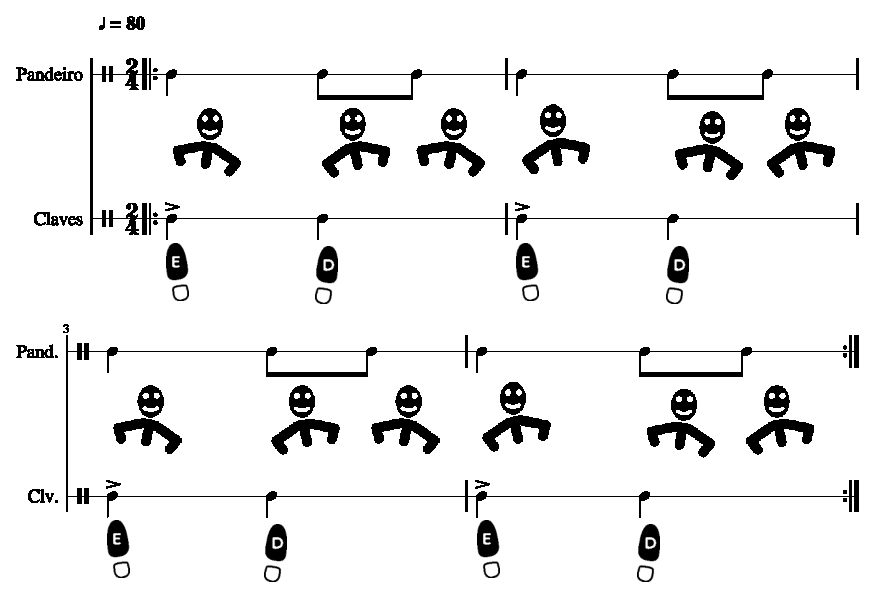
\includegraphics[width=\bodyboxsize]{chapters/cap-body-isolation/bodycontrol1-poliritmia-1.eps}
\caption{Exercício de polirritmia.}
\label{fig:bodycontrol1-poliritmia-1}
\end{figure}



